%\documentclass[amsmath,table,sans,amsfonts, handout]{beamer}
\documentclass[amsmath,table,sans,amsfonts]{beamer}
\usepackage[T1]{fontenc}
%%\usepackage{beamerthemeshadow}
%%\usepackage[headheight=1pt,footheight=10pt]{beamerthemeboxes}
%%\addfootboxtemplate{\color{structure!80}}{\color{white}\tiny \hfill Karl Svozil (TU Vienna)\hfill}
%%\addfootboxtemplate{\color{structure!65}}{\color{white}\tiny \hfill mur.sat \hfill}
%%\addfootboxtemplate{\color{structure!50}}{\color{white}\tiny \hfill Graz, 2010-12-11\hfill}
%\usepackage[dark]{beamerthemesidebar}
%\usepackage[headheight=24pt,footheight=12pt]{beamerthemesplit}
%\usepackage{beamerthemesplit}
%\usepackage[bar]{beamerthemetree}
\usepackage{graphicx}

%Global Background must be put in preamble
{%
%\usebackgroundtemplate%      \includegraphics[width=\paperwidth,height=\paperheight]{HaK-Urkaos-da}%
}
 \setbeamercolor{background canvas}{bg=black}

\usepackage{eepic}
%\usepackage[usenames]{color}
%\newcommand{\Red}{\color{Red}}  %(VERY-Approx.PANTONE-RED)
%\newcommand{\Green}{\color{Green}}  %(VERY-Approx.PANTONE-GREEN)


%\RequirePackage[german]{babel}
%\selectlanguage{german}
%\RequirePackage[isolatin]{inputenc}

%\pgfdeclareimage[height=0.5cm]{logo}{tu-logo}
%\logo{\pgfuseimage{logo}}
\beamertemplatetriangleitem
%\beamertemplateballitem

\beamerboxesdeclarecolorscheme{alert}{red}{red!15!averagebackgroundcolor}
%\begin{beamerboxesrounded}[scheme=alert,shadow=true]{}
%\end{beamerboxesrounded}

%\beamersetaveragebackground{yellow!10}

%\beamertemplatecircleminiframe

\newtheorem{question}{Question}
\newtheorem{conjecture}[question]{Principle}
\newtheorem{challenge}[question]{Challenge}

\usepackage{tikz}
\usetikzlibrary{calc,decorations.pathreplacing,decorations.markings}





        \definecolor{orange(webcolor)}{rgb}{1.0, 0.65, 0.0}
\setbeamercolor{normal text}{fg=yellow}
\setbeamercolor{structure}{fg=yellow}




\begin{document}




\title{\bf \textcolor{orange!100}{Probabilities on logics with lean sets of two-valued states}}
\subtitle{\textcolor{orange!100}{\small http://tph.tuwien.ac.at/$\sim$svozil/publ/2017-Svozil-Cordoba-pres.pdf
%\\
%Nature-Springer, in press 2017; drafts on demand
}}
\author{\textcolor{orange!100}{Karl Svozil}}
\institute{\textcolor{orange!100}{ITP/Vienna University of Technology, Austria\\
\& CS/University of Auckland, NZ  \\
svozil@tuwien.ac.at
}
%{\tiny Disclaimer: Die hier vertretenen Meinungen des Autors verstehen sich als Diskussionsbeitr�ge und decken sich nicht notwendigerweise mit den Positionen der Technischen Universit�t Wien oder deren Vertreter.}
}
\date{\textcolor{orange!100}{Cordoba, Argentina, Nov 29th, 2017}}

\maketitle

% \frame{
% \frametitle{}
%
% }




 \frame{
 \frametitle{Some questions one could ask, and answers one might expect}

\begin{itemize}
%\pause
\item
Does a(n empirical) structure of propositions (logic) induce a probability?  No!

\item
What kind of non-Boolean (non-classical) structure of propositions can one imagine?
\begin{itemize}
%\pause
\item
Classical Boolean algebras

\item
Wright's generalized urn model (partition logics)

\item
Moore's finite automaton state identification problem (partition logics)

\item
quantum logics (Hilbert lattices)

\item
general logics constructed by the pasting of Boolean subalgebras (contexts, blocks)

\end{itemize}

\item
What criteria/axioms to assume for probabilities? Gleason-type frame functions: additivity of mutual exclusive events, totally  (im)probable events have probability 0 and 1, respectively.


\end{itemize}



 }






\frame{
\frametitle{Geometric strategies to classical probabilities
}

\begin{itemize}
%\pause
\item
Froissart (1981), Pitowsky (1986), Tsirelson (1993): geometric interpretation of probability distributions
as surface of a convex polytope ``spanned''
by vertices aka ``mutually exclusive extreme cases.''


\begin{itemize}
%\pause
\item
The vertices are encoded by two-valued states on the logic.

\item
The face (in)equalities indicating ``inside-outside relations'' are
very similar to Boole's ``conditions of possible experience'' (1854,1862).


\item
The  {\em hull problem} of finding these faces is NP-complete in the number of vertices.


\end{itemize}
\end{itemize}
}

\frame{
\frametitle{Geometric strategies to (quasi)classical probabilities
}

\begin{itemize}

\item
I suggest to generalize these methods for (quasi)classical models
to situations when there are ``enough'' [i.e., the set of two-valued states is separating (Kochen-Specker, 1967)]
two-valued states on the logic.

\item
These can be used to finding (quasi)classical probability  distributions on, say, partition logics
(from generalized urn models or finite automaton state identification).


\end{itemize}

}

\begin{frame}[fragile]{Example I: Pentagon logic}

\begin{center}
%TexCad Options
%\grade{\off}
%\emlines{\off}
%\beziermacro{\off}
%\reduce{\on}
%\snapping{\off}
%\quality{0.20}
%\graddiff{0.01}
%\snapasp{1}
%\zoom{1.00}
\unitlength 0.16mm
%\thicklines %\linethickness{1pt}
\allinethickness{2.1pt}
\begin{picture}(230,200)(-110,-100)
%\emline(31,-95.25)(100,0)
\multiput(31,-95.25)(.033724340176,.046554252199){2046}{\color{cyan}\line(0,1){.046554252199}}
%\end
%\emline(100,0)(31,95)
\multiput(100,0)(-.033724340176,.046432062561){2046}{\color{magenta}\line(0,1){.046432062561}}
%\end
%\emline(31,95)(-81,58.75)
\multiput(31,95)(-.10418604651,-.03372093023){1075}{\color{blue}\line(-1,0){.10418604651}}
%\end
\put(-81,58.75){\color{red}\line(0,-1){117.75}}
%\emline(-81,-59)(30.75,-95.5)
\multiput(-81,-59)(.10328096118,-.03373382625){1082}{\color{green}\line(1,0){.10328096118}}
%\end
%
\put( 30.9017 , 95.1057){\color{magenta}\circle{15.00}}
\put( 30.9017 , 95.1057){\color{blue}\circle{6}} %a_1
\put( 30.9017 , 95.1057){\color{blue}\circle{1}} %a_1
\put( 55.9017 , 95.1057){\makebox(0,0)[cc]{$a_1$}}
%
\put( 65.4509,47.5529){\color{magenta}\circle{9}}  %a_2
\put( 90.4509,47.5529){\makebox(0,0)[cc]{$a_2$}}
%
%
\put(100,0){\color{cyan}\circle{15.00}}
\put(100,0){\color{magenta}\circle{6}}    %a_3
\put(100,0){\color{magenta}\circle{1}}    %a_3
\put(120,0){\makebox(0,0)[cc]{$a_3$}}
%
\put( 65.4509,-47.5529){\color{cyan}\circle{9}}  %a_4
\put( 90.4509,-47.5529){\makebox(0,0)[cc]{$a_4$}}
%
\put( 30.9017 , -95.1057){\color{green}\circle{15.00}}
\put( 30.9017 , -95.1057){\color{cyan}\circle{6}}  %a_5
\put( 30.9017 , -95.1057){\color{cyan}\circle{1}}  %a_5
\put( 55.9017 , -95.1057){\makebox(0,0)[cc]{$a_5$}}
%
\put( -25,-76.9421){\color{green}\circle{9}}         %a_6
\put( -40,-90.9421){\makebox(0,0)[cc]{$a_6$}}
%
\put( -80.9017 , -58.7785){\color{red}\circle{15.00}}
\put( -80.9017 , -58.7785){\color{green}\circle{6}}   %a_7
\put( -80.9017 , -58.7785){\color{green}\circle{1}}   %a_7
\put( -105.9017 , -58.7785){\makebox(0,0)[cc]{$a_7$}}
%
\put(-80.9017,0){\color{red}\circle{9}}           %a_8
\put(-105.9017,0){\makebox(0,0)[cc]{$a_8$}}
%
\put(-80.9017 , 58.7785){\color{blue}\circle{15}}
\put(-80.9017 , 58.7785){\color{red}\circle{6}}     %a_9
\put(-80.9017 , 58.7785){\color{red}\circle{1}}     %a_9
\put(-105.9017 , 58.7785){\makebox(0,0)[cc]{$a_9$}}
%
\put( -25,76.9421){\color{blue}\circle{9}}         %a_10
\put( -40,90.9421){\makebox(0,0)[cc]{$a_{10}$}}
\end{picture}
\end{center}

\end{frame}

\begin{frame}[fragile]{Example I: two-valued states on the pentagon logic (Wright, 1978)}

 \begin{center}
 \begin{tabular}{ccccccccccc}
\#
&
$a_1$&
$a_2$&
$a_3$&
$a_4$&
$a_5$&
$a_6$&
$a_7$&
$a_8$&
$a_9$&
$a_{10}$
\\
\hline
$v_1$&1&  0&  0& 1&  0& 1&  0& 1&  0&  0 \\
$v_2$&1&  0&  0&  0& 1&  0&  0& 1&  0&  0\\
$v_3$&1&  0&  0& 1&  0&  0& 1&  0&  0&  0\\
$v_4$&0&  0& 1&  0&  0& 1&  0& 1&  0& 1\\
$v_5$&0&  0& 1&  0&  0&  0& 1&  0&  0& 1\\
$v_6$&0&  0& 1&  0&  0& 1&  0&  0& 1&  0\\
$v_7$&0& 1&  0&  0& 1&  0&  0& 1&  0& 1\\
$v_8$&0& 1&  0&  0& 1&  0&  0&  0& 1&  0\\
$v_9$&0& 1&  0& 1&  0&  0& 1&  0&  0& 1\\
$v_{10}$&0& 1&  0& 1&  0& 1&  0&  0& 1&  0\\
$v_{11}$&0& 1&  0& 1&  0& 1&  0& 1&  0& 1 \\
\hline
$v_e$&$\frac{1}{2}$& 0&  $\frac{1}{2}$& 0&  $\frac{1}{2}$& 0&  $\frac{1}{2}$& 0&  $\frac{1}{2}$& 0
 \end{tabular}
 \end{center}


\end{frame}





\begin{frame}[fragile]{Example I: two-valued states on the pentagon logic (Wright, 1978)}

 \begin{center}
\begin{tabular}{cccc}
%TexCad Options
%\grade{\off}
%\emlines{\off}
%\beziermacro{\off}
%\reduce{\on}
%\snapping{\off}
%\quality{0.20}
%\graddiff{0.01}
%\snapasp{1}
%\zoom{1.00}
\unitlength 0.1mm
%\thicklines %\linethickness{1pt}
\allinethickness{1.5pt}
\begin{picture}(230,200)(-110,-100)
\put(0,0){\makebox(0,0)[cc]{\large $v_1$}}
%\emline(31,-95.25)(100,0)
\multiput(31,-95.25)(1.2,1.6565){58}{\color{cyan}\line(0,1){.1656521739}}
%\end
%\emline(100,0)(31,95)
\multiput(100,0)(-1.2,1.6522){58}{\color{magenta}\line(0,1){.1652173913}}
%\end
%\emline(31,95)(-81,58.75)
\multiput(31,95)(-3.69637,-1.19637){30}{\color{blue}\line(-1,0){.3696369637}}
%\end
%\put(-81,58.75){\color{red}\line(0,-1){117.75}}
\multiput(-81,59)(0,-2){60}{\color{red}\line(0,-1){0.33}}
%\emline(-81,-59)(30.75,-95.5)
\multiput(-81,-59)(3.664,-1.1967){31}{\color{green}\line(1,0){.3663934426}}
%\end
%
\put( 30.9017 , 95.1057){\circle{4}} %a_1
\put( 65.4509,-47.5529){\circle{4}}  %a_4
\put( -25,-76.9421){\circle{4}}         %a_6
\put(-80.9017,0){\circle{4}}           %a_8
\put( 30.9017 , 95.1057){\circle{10}} %a_1
\put( 65.4509,-47.5529){\circle{10}}  %a_4
\put( -25,-76.9421){\circle{10}}         %a_6
\put(-80.9017,0){\circle{10}}           %a_8
\put( 30.9017 , 95.1057){\circle{18}} %a_1
\put( 65.4509,-47.5529){\circle{18}}  %a_4
\put( -25,-76.9421){\circle{18}}         %a_6
\put(-80.9017,0){\circle{18}}           %a_8
\end{picture}
&
%TexCad Options
%\grade{\off}
%\emlines{\off}
%\beziermacro{\off}
%\reduce{\on}
%\snapping{\off}
%\quality{0.20}
%\graddiff{0.01}
%\snapasp{1}
%\zoom{1.00}
\unitlength 0.1mm
%\thicklines %\linethickness{1pt}
\allinethickness{1.5pt}
\begin{picture}(230,200)(-110,-100)
\put(0,0){\makebox(0,0)[cc]{\large $v_2$}}
%\emline(31,-95.25)(100,0)
\multiput(31,-95.25)(1.2,1.6565){58}{\color{cyan}\line(0,1){.1656521739}}
%\end
%\emline(100,0)(31,95)
\multiput(100,0)(-1.2,1.6522){58}{\color{magenta}\line(0,1){.1652173913}}
%\end
%\emline(31,95)(-81,58.75)
\multiput(31,95)(-3.69637,-1.19637){30}{\color{blue}\line(-1,0){.3696369637}}
%\end
\multiput(-81,59)(0,-2){60}{\color{red}\line(0,-1){0.33}}
%\emline(-81,-59)(30.75,-95.5)
\multiput(-81,-59)(3.664,-1.1967){31}{\color{green}\line(1,0){.3663934426}}
%\end
%
\put( 30.9017 , 95.1057){\circle{4}} %a_1
\put( 30.9017 , -95.1057){\circle{4}}  %a_5
\put(-80.9017,0){\circle{4}}           %a_8
\put( 30.9017 , 95.1057){\circle{10}} %a_1
\put( 30.9017 , -95.1057){\circle{10}}  %a_5
\put(-80.9017,0){\circle{10}}           %a_8
\put( 30.9017 , 95.1057){\circle{18}} %a_1
\put( 30.9017 , -95.1057){\circle{18}}  %a_5
\put(-80.9017,0){\circle{18}}           %a_8
\end{picture}
&
%TexCad Options
%\grade{\off}
%\emlines{\off}
%\beziermacro{\off}
%\reduce{\on}
%\snapping{\off}
%\quality{0.20}
%\graddiff{0.01}
%\snapasp{1}
%\zoom{1.00}
\unitlength 0.1mm
%\thicklines %\linethickness{1pt}
\allinethickness{1.5pt}
\begin{picture}(230,200)(-110,-100)
\put(0,0){\makebox(0,0)[cc]{\large $v_3$}}
%\emline(31,-95.25)(100,0)
\multiput(31,-95.25)(1.2,1.6565){58}{\color{cyan}\line(0,1){.1656521739}}
%\end
%\emline(100,0)(31,95)
\multiput(100,0)(-1.2,1.6522){58}{\color{magenta}\line(0,1){.1652173913}}
%\end
%\emline(31,95)(-81,58.75)
\multiput(31,95)(-3.69637,-1.19637){30}{\color{blue}\line(-1,0){.3696369637}}
%\end
\multiput(-81,59)(0,-2){60}{\color{red}\line(0,-1){0.33}}
%\emline(-81,-59)(30.75,-95.5)
\multiput(-81,-59)(3.664,-1.1967){31}{\color{green}\line(1,0){.3663934426}}
%\end
%
\put( 30.9017 , 95.1057){\circle{4}} %a_1
\put( 65.4509,-47.5529){\circle{4}}  %a_4
\put( -80.9017 , -58.7785){\circle{4}}   %a_7
\put( 30.9017 , 95.1057){\circle{10}} %a_1
\put( 65.4509,-47.5529){\circle{10}}  %a_4
\put( -80.9017 , -58.7785){\circle{10}}   %a_7
\put( 30.9017 , 95.1057){\circle{18}} %a_1
\put( 65.4509,-47.5529){\circle{18}}  %a_4
\put( -80.9017 , -58.7785){\circle{18}}   %a_7
\end{picture}
&
%TexCad Options
%\grade{\off}
%\emlines{\off}
%\beziermacro{\off}
%\reduce{\on}
%\snapping{\off}
%\quality{0.20}
%\graddiff{0.01}
%\snapasp{1}
%\zoom{1.00}
\unitlength 0.1mm
%\thicklines %\linethickness{1pt}
\allinethickness{1.5pt}
\begin{picture}(230,200)(-110,-100)
\put(0,0){\makebox(0,0)[cc]{\large $v_4$}}
%\emline(31,-95.25)(100,0)
\multiput(31,-95.25)(1.2,1.6565){58}{\color{cyan}\line(0,1){.1656521739}}
%\end
%\emline(100,0)(31,95)
\multiput(100,0)(-1.2,1.6522){58}{\color{magenta}\line(0,1){.1652173913}}
%\end
%\emline(31,95)(-81,58.75)
\multiput(31,95)(-3.69637,-1.19637){30}{\color{blue}\line(-1,0){.3696369637}}
%\end
\multiput(-81,59)(0,-2){60}{\color{red}\line(0,-1){0.33}}
%\emline(-81,-59)(30.75,-95.5)
\multiput(-81,-59)(3.664,-1.1967){31}{\color{green}\line(1,0){.3663934426}}
%\end
%
\put(100,0){\circle{4}}    %a_3
\put( -25,-76.9421){\circle{4}}         %a_6
\put(-80.9017,0){\circle{4}}           %a_8
\put( -25,76.9421){\circle{4}}         %a_10
\put(100,0){\circle{10}}    %a_3
\put( -25,-76.9421){\circle{10}}         %a_6
\put(-80.9017,0){\circle{10}}           %a_8
\put( -25,76.9421){\circle{10}}         %a_10
\put(100,0){\circle{18}}    %a_3
\put( -25,-76.9421){\circle{18}}         %a_6
\put(-80.9017,0){\circle{18}}           %a_8
\put( -25,76.9421){\circle{18}}         %a_10
\end{picture}
\\
%TexCad Options
%\grade{\off}
%\emlines{\off}
%\beziermacro{\off}
%\reduce{\on}
%\snapping{\off}
%\quality{0.20}
%\graddiff{0.01}
%\snapasp{1}
%\zoom{1.00}
\unitlength 0.1mm
%\thicklines %\linethickness{1pt}
\allinethickness{1.5pt}
\begin{picture}(230,200)(-110,-100)
\put(0,0){\makebox(0,0)[cc]{\large $v_5$}}
%\emline(31,-95.25)(100,0)
\multiput(31,-95.25)(1.2,1.6565){58}{\color{cyan}\line(0,1){.1656521739}}
%\end
%\emline(100,0)(31,95)
\multiput(100,0)(-1.2,1.6522){58}{\color{magenta}\line(0,1){.1652173913}}
%\end
%\emline(31,95)(-81,58.75)
\multiput(31,95)(-3.69637,-1.19637){30}{\color{blue}\line(-1,0){.3696369637}}
%\end
\multiput(-81,59)(0,-2){60}{\color{red}\line(0,-1){0.33}}
%\emline(-81,-59)(30.75,-95.5)
\multiput(-81,-59)(3.664,-1.1967){31}{\color{green}\line(1,0){.3663934426}}
%\end
%
\put(100,0){\circle{4}}    %a_3
\put( -80.9017 , -58.7785){\circle{4}}   %a_7
\put( -25,76.9421){\circle{4}}         %a_10
\put(100,0){\circle{10}}    %a_3
\put( -80.9017 , -58.7785){\circle{10}}   %a_7
\put( -25,76.9421){\circle{10}}         %a_10
\put(100,0){\circle{18}}    %a_3
\put( -80.9017 , -58.7785){\circle{18}}   %a_7
\put( -25,76.9421){\circle{18}}         %a_10
\end{picture}
&
%TexCad Options
%\grade{\off}
%\emlines{\off}
%\beziermacro{\off}
%\reduce{\on}
%\snapping{\off}
%\quality{0.20}
%\graddiff{0.01}
%\snapasp{1}
%\zoom{1.00}
\unitlength 0.1mm
%\thicklines %\linethickness{1pt}
\allinethickness{1.5pt}
\begin{picture}(230,200)(-110,-100)
\put(0,0){\makebox(0,0)[cc]{\large $v_6$}}
%\emline(31,-95.25)(100,0)
\multiput(31,-95.25)(1.2,1.6565){58}{\color{cyan}\line(0,1){.1656521739}}
%\end
%\emline(100,0)(31,95)
\multiput(100,0)(-1.2,1.6522){58}{\color{magenta}\line(0,1){.1652173913}}
%\end
%\emline(31,95)(-81,58.75)
\multiput(31,95)(-3.69637,-1.19637){30}{\color{blue}\line(-1,0){.3696369637}}
%\end
\multiput(-81,59)(0,-2){60}{\color{red}\line(0,-1){0.33}}
%\emline(-81,-59)(30.75,-95.5)
\multiput(-81,-59)(3.664,-1.1967){31}{\color{green}\line(1,0){.3663934426}}
%\end
%
\put(100,0){\circle{4}}    %a_3
\put( -25,-76.9421){\circle{4}}         %a_6
\put(-80.9017 , 58.7785){\circle{4}}     %a_9
\put(100,0){\circle{10}}    %a_3
\put( -25,-76.9421){\circle{10}}         %a_6
\put(-80.9017 , 58.7785){\circle{10}}     %a_9
\put(100,0){\circle{18}}    %a_3
\put( -25,-76.9421){\circle{18}}         %a_6
\put(-80.9017 , 58.7785){\circle{18}}     %a_9
\end{picture}
&
%TexCad Options
%\grade{\off}
%\emlines{\off}
%\beziermacro{\off}
%\reduce{\on}
%\snapping{\off}
%\quality{0.20}
%\graddiff{0.01}
%\snapasp{1}
%\zoom{1.00}
\unitlength 0.1mm
%\thicklines %\linethickness{1pt}
\allinethickness{1.5pt}
\begin{picture}(230,200)(-110,-100)
\put(0,0){\makebox(0,0)[cc]{\large $v_7$}}
%\emline(31,-95.25)(100,0)
\multiput(31,-95.25)(1.2,1.6565){58}{\color{cyan}\line(0,1){.1656521739}}
%\end
%\emline(100,0)(31,95)
\multiput(100,0)(-1.2,1.6522){58}{\color{magenta}\line(0,1){.1652173913}}
%\end
%\emline(31,95)(-81,58.75)
\multiput(31,95)(-3.69637,-1.19637){30}{\color{blue}\line(-1,0){.3696369637}}
%\end
\multiput(-81,59)(0,-2){60}{\color{red}\line(0,-1){0.33}}
%\emline(-81,-59)(30.75,-95.5)
\multiput(-81,-59)(3.664,-1.1967){31}{\color{green}\line(1,0){.3663934426}}
%\end
%
\put( 65.4509,47.5529){\circle{4}}  %a_2
\put( 30.9017 , -95.1057){\circle{4}}  %a_5
\put(-80.9017,0){\circle{4}}           %a_8
\put( -25,76.9421){\circle{4}}         %a_10
\put( 65.4509,47.5529){\circle{10}}  %a_2
\put( 30.9017 , -95.1057){\circle{10}}  %a_5
\put(-80.9017,0){\circle{10}}           %a_8
\put( -25,76.9421){\circle{10}}         %a_10
\put( 65.4509,47.5529){\circle{18}}  %a_2
\put( 30.9017 , -95.1057){\circle{18}}  %a_5
\put(-80.9017,0){\circle{18}}           %a_8
\put( -25,76.9421){\circle{18}}         %a_10
\end{picture}
&
%TexCad Options
%\grade{\off}
%\emlines{\off}
%\beziermacro{\off}
%\reduce{\on}
%\snapping{\off}
%\quality{0.20}
%\graddiff{0.01}
%\snapasp{1}
%\zoom{1.00}
\unitlength 0.1mm
%\thicklines %\linethickness{1pt}
\allinethickness{1.5pt}
\begin{picture}(230,200)(-110,-100)
\put(0,0){\makebox(0,0)[cc]{\large $v_8$}}
%\emline(31,-95.25)(100,0)
\multiput(31,-95.25)(1.2,1.6565){58}{\color{cyan}\line(0,1){.1656521739}}
%\end
%\emline(100,0)(31,95)
\multiput(100,0)(-1.2,1.6522){58}{\color{magenta}\line(0,1){.1652173913}}
%\end
%\emline(31,95)(-81,58.75)
\multiput(31,95)(-3.69637,-1.19637){30}{\color{blue}\line(-1,0){.3696369637}}
%\end
\multiput(-81,59)(0,-2){60}{\color{red}\line(0,-1){0.33}}
%\emline(-81,-59)(30.75,-95.5)
\multiput(-81,-59)(3.664,-1.1967){31}{\color{green}\line(1,0){.3663934426}}
%\end
%
\put( 65.4509,47.5529){\circle{4}}  %a_2
\put( 30.9017 , -95.1057){\circle{4}}  %a_5
\put(-80.9017 , 58.7785){\circle{4}}     %a_9
\put( 65.4509,47.5529){\circle{10}}  %a_2
\put( 30.9017 , -95.1057){\circle{10}}  %a_5
\put(-80.9017 , 58.7785){\circle{10}}     %a_9
\put( 65.4509,47.5529){\circle{18}}  %a_2
\put( 30.9017 , -95.1057){\circle{18}}  %a_5
\put(-80.9017 , 58.7785){\circle{18}}     %a_9
\end{picture}
\\
%TexCad Options
%\grade{\off}
%\emlines{\off}
%\beziermacro{\off}
%\reduce{\on}
%\snapping{\off}
%\quality{0.20}
%\graddiff{0.01}
%\snapasp{1}
%\zoom{1.00}
\unitlength 0.1mm
%\thicklines %\linethickness{1pt}
\allinethickness{1.5pt}
\begin{picture}(230,200)(-110,-100)
\put(0,0){\makebox(0,0)[cc]{\large $v_9$}}
%\emline(31,-95.25)(100,0)
\multiput(31,-95.25)(1.2,1.6565){58}{\color{cyan}\line(0,1){.1656521739}}
%\end
%\emline(100,0)(31,95)
\multiput(100,0)(-1.2,1.6522){58}{\color{magenta}\line(0,1){.1652173913}}
%\end
%\emline(31,95)(-81,58.75)
\multiput(31,95)(-3.69637,-1.19637){30}{\color{blue}\line(-1,0){.3696369637}}
%\end
\multiput(-81,59)(0,-2){60}{\color{red}\line(0,-1){0.33}}
%\emline(-81,-59)(30.75,-95.5)
\multiput(-81,-59)(3.664,-1.1967){31}{\color{green}\line(1,0){.3663934426}}
%\end
%
\put( 65.4509,47.5529){\circle{4}}  %a_2
\put( 65.4509,-47.5529){\circle{4}}  %a_4
\put( -80.9017 , -58.7785){\circle{4}}   %a_7
\put( -25,76.9421){\circle{4}}         %a_10
\put( 65.4509,47.5529){\circle{10}}  %a_2
\put( 65.4509,-47.5529){\circle{10}}  %a_4
\put( -80.9017 , -58.7785){\circle{10}}   %a_7
\put( -25,76.9421){\circle{10}}         %a_10
\put( 65.4509,47.5529){\circle{18}}  %a_2
\put( 65.4509,-47.5529){\circle{18}}  %a_4
\put( -80.9017 , -58.7785){\circle{18}}   %a_7
\put( -25,76.9421){\circle{18}}         %a_10
\end{picture}
&
%TexCad Options
%\grade{\off}
%\emlines{\off}
%\beziermacro{\off}
%\reduce{\on}
%\snapping{\off}
%\quality{0.20}
%\graddiff{0.01}
%\snapasp{1}
%\zoom{1.00}
\unitlength 0.1mm
%\thicklines %\linethickness{1pt}
\allinethickness{1.5pt}
\begin{picture}(230,200)(-110,-100)
\put(0,0){\makebox(0,0)[cc]{\large $v_{10}$}}
%\emline(31,-95.25)(100,0)
\multiput(31,-95.25)(1.2,1.6565){58}{\color{cyan}\line(0,1){.1656521739}}
%\end
%\emline(100,0)(31,95)
\multiput(100,0)(-1.2,1.6522){58}{\color{magenta}\line(0,1){.1652173913}}
%\end
%\emline(31,95)(-81,58.75)
\multiput(31,95)(-3.69637,-1.19637){30}{\color{blue}\line(-1,0){.3696369637}}
%\end
\multiput(-81,59)(0,-2){60}{\color{red}\line(0,-1){0.33}}
%\emline(-81,-59)(30.75,-95.5)
\multiput(-81,-59)(3.664,-1.1967){31}{\color{green}\line(1,0){.3663934426}}
%\end
%
\put( 65.4509,47.5529){\circle{4}}  %a_2
\put( 65.4509,-47.5529){\circle{4}}  %a_4
\put( -25,-76.9421){\circle{4}}         %a_6
\put(-80.9017 , 58.7785){\circle{4}}     %a_9
\put( 65.4509,47.5529){\circle{10}}  %a_2
\put( 65.4509,-47.5529){\circle{10}}  %a_4
\put( -25,-76.9421){\circle{10}}         %a_6
\put(-80.9017 , 58.7785){\circle{10}}     %a_9
\put( 65.4509,47.5529){\circle{18}}  %a_2
\put( 65.4509,-47.5529){\circle{18}}  %a_4
\put( -25,-76.9421){\circle{18}}         %a_6
\put(-80.9017 , 58.7785){\circle{18}}     %a_9
\end{picture}
%
&
%TexCad Options
%\grade{\off}
%\emlines{\off}
%\beziermacro{\off}
%\reduce{\on}
%\snapping{\off}
%\quality{0.20}
%\graddiff{0.01}
%\snapasp{1}
%\zoom{1.00}
\unitlength 0.1mm
%\thicklines %\linethickness{1pt}
\allinethickness{1.5pt}
\begin{picture}(230,200)(-110,-100)
\put(0,0){\makebox(0,0)[cc]{\large $v_{11}$}}
%\emline(31,-95.25)(100,0)
\multiput(31,-95.25)(1.2,1.6565){58}{\color{cyan}\line(0,1){.1656521739}}
%\end
%\emline(100,0)(31,95)
\multiput(100,0)(-1.2,1.6522){58}{\color{magenta}\line(0,1){.1652173913}}
%\end
%\emline(31,95)(-81,58.75)
\multiput(31,95)(-3.69637,-1.19637){30}{\color{blue}\line(-1,0){.3696369637}}
%\end
\multiput(-81,59)(0,-2){60}{\color{red}\line(0,-1){0.33}}
%\emline(-81,-59)(30.75,-95.5)
\multiput(-81,-59)(3.664,-1.1967){31}{\color{green}\line(1,0){.3663934426}}
%\end
%
\put( 65.4509,47.5529){\circle{4}}  %a_2
\put( 65.4509,-47.5529){\circle{4}}  %a_4
\put( -25,-76.9421){\circle{4}}         %a_6
\put(-80.9017,0){\circle{4}}           %a_8
\put( -25,76.9421){\circle{4}}         %a_10
\put( 65.4509,47.5529){\circle{10}}  %a_2
\put( 65.4509,-47.5529){\circle{10}}  %a_4
\put( -25,-76.9421){\circle{10}}         %a_6
\put(-80.9017,0){\circle{10}}           %a_8
\put( -25,76.9421){\circle{10}}         %a_10
\put( 65.4509,47.5529){\circle{18}}  %a_2
\put( 65.4509,-47.5529){\circle{18}}  %a_4
\put( -25,-76.9421){\circle{18}}         %a_6
\put(-80.9017,0){\circle{18}}           %a_8
\put( -25,76.9421){\circle{18}}         %a_10
\end{picture}
&
%TexCad Options
%\grade{\off}
%\emlines{\off}
%\beziermacro{\off}
%\reduce{\on}
%\snapping{\off}
%\quality{0.20}
%\graddiff{0.01}
%\snapasp{1}
%\zoom{1.00}
\unitlength 0.1mm
%\thicklines %\linethickness{1pt}
\allinethickness{1.5pt}
\begin{picture}(230,200)(-110,-100)
\put(0,0){\makebox(0,0)[cc]{\large $v_e$}}
%\emline(31,-95.25)(100,0)
\multiput(31,-95.25)(1.2,1.6565){58}{\color{cyan}\line(0,1){.1656521739}}
%\end
%\emline(100,0)(31,95)
\multiput(100,0)(-1.2,1.6522){58}{\color{magenta}\line(0,1){.1652173913}}
%\end
%\emline(31,95)(-81,58.75)
\multiput(31,95)(-3.69637,-1.19637){30}{\color{blue}\line(-1,0){.3696369637}}
%\end
\multiput(-81,59)(0,-2){60}{\color{red}\line(0,-1){0.33}}
%\emline(-81,-59)(30.75,-95.5)
\multiput(-81,-59)(3.664,-1.1967){31}{\color{green}\line(1,0){.3663934426}}
%\end
%
%
\put( 30.9017 , 95.1057){\color{white}\circle{4}} %a_1
\put(100,0){\color{white}\circle{4}}    %a_3
\put( 30.9017 , -95.1057){\color{white}\circle{4}}  %a_5
\put( -80.9017 , -58.7785){\color{white}\circle{4}}   %a_7
\put(-80.9017 , 58.7785){\color{white}\circle{4}}     %a_9
\put( 30.9017 , 95.1057){\color{white}\circle{10}} %a_1
\put(100,0){\color{white}\circle{10}}    %a_3
\put( 30.9017 , -95.1057){\color{white}\circle{10}}  %a_5
\put( -80.9017 , -58.7785){\color{white}\circle{10}}   %a_7
\put(-80.9017 , 58.7785){\color{white}\circle{10}}     %a_9
\put( 30.9017 , 95.1057){\circle{18}} %a_1
\put(100,0){\circle{18}}    %a_3
\put( 30.9017 , -95.1057){\circle{18}}  %a_5
\put( -80.9017 , -58.7785){\circle{18}}   %a_7
\put(-80.9017 , 58.7785){\circle{18}}     %a_9
\end{picture}
\end{tabular}
 \end{center}
\end{frame}



\begin{frame}[fragile]{Example I: Probabilities on partition logics from two-valued states on the pentagon logic -- with
$\lambda_i \ge 0$, $i=1,\ldots 11$, $\sum_{i=1}^{11} \lambda_i = 1$}

 \begin{center}
%TexCad Options
%\grade{\off}
%\emlines{\off}
%\beziermacro{\off}
%\reduce{\on}
%\snapping{\off}
%\quality{0.20}
%\graddiff{0.01}
%\snapasp{1}
%\zoom{1.00}
\unitlength 0.12mm
%\thicklines %\linethickness{1pt}
\allinethickness{2.1pt}
\begin{picture}(230,250)(-110,-115)
%\emline(31,-95.25)(100,0)
\multiput(31,-95.25)(.033724340176,.046554252199){2046}{\color{cyan}\line(0,1){.046554252199}}
%\end
%\emline(100,0)(31,95)
\multiput(100,0)(-.033724340176,.046432062561){2046}{\color{magenta}\line(0,1){.046432062561}}
%\end
%\emline(31,95)(-81,58.75)
\multiput(31,95)(-.10418604651,-.03372093023){1075}{\color{blue}\line(-1,0){.10418604651}}
%\end
\put(-81,58.75){\color{red}\line(0,-1){117.75}}
%\emline(-81,-59)(30.75,-95.5)
\multiput(-81,-59)(.10328096118,-.03373382625){1082}{\color{green}\line(1,0){.10328096118}}
%\end
%
\put( 30.9017 , 95.1057){\color{magenta}\circle{15.00}}
\put( 30.9017 , 95.1057){\color{blue}\circle{6}} %a_1
\put( 30.9017 , 95.1057){\color{blue}\circle{1.20}} %a_1
\put( 55.9017 , 95.1057){\makebox(0,0)[lc]{$\lambda_1 + \lambda_2 + \lambda_3$}}
%
\put( 65.4509,47.5529){\color{magenta}\circle{12.00}}  %a_2
\put( 65.4509,47.5529){\color{magenta}\circle{5.00}}  %a_2
\put( 90.4509,47.5529){\makebox(0,0)[lc]{$\lambda_7 + \lambda_8 + \lambda_9 + \lambda_{10} + \lambda_{11}$}}
%
%
\put(100,0){\color{cyan}\circle{15.00}}
\put(100,0){\color{magenta}\circle{6}}    %a_3
\put(100,0){\color{magenta}\circle{1.20}}    %a_3
\put(120,0){\makebox(0,0)[lc]{$\lambda_4 + \lambda_5 + \lambda_6$}}
%
\put( 65.4509,-47.5529){\color{cyan}\circle{12.00}}  %a_4
\put( 65.4509,-47.5529){\color{cyan}\circle{5.00}}  %a_4
\put( 90.4509,-47.5529){\makebox(0,0)[lc]{$\lambda_1 + \lambda_3 + \lambda_9 + \lambda_{10} + \lambda_{11}$}}
%
\put( 30.9017 , -95.1057){\color{green}\circle{15.00}}
\put( 30.9017 , -95.1057){\color{cyan}\circle{6}}  %a_5
\put( 30.9017 , -95.1057){\color{cyan}\circle{1.20}}  %a_5
\put(55.9017 , -95.1057){\makebox(0,0)[lc]{$\lambda_2 + \lambda_7 + \lambda_8$}}
%
\put( -25,-76.9421){\color{green}\circle{12.00}}         %a_6
\put( -25,-76.9421){\color{green}\circle{5.00}}         %a_6
\put( -40,-90.9421){\makebox(0,0)[rc]{$\lambda_1 + \lambda_4 + \lambda_6 + \lambda_{10} + \lambda_{11}$}}
%
\put( -80.9017 , -58.7785){\color{red}\circle{15.00}}
\put( -80.9017 , -58.7785){\color{green}\circle{6}}   %a_7
\put( -80.9017 , -58.7785){\color{green}\circle{1.20}}   %a_7
\put( -105.9017 , -58.7785){\makebox(0,0)[rc]{$\lambda_3 + \lambda_5 + \lambda_9 + \lambda_3$}}
%
\put(-80.9017,0){\color{red}\circle{12.00}}           %a_8
\put(-80.9017,0){\color{red}\circle{5.00}}           %a_8
\put(-105.9017,0){\makebox(0,0)[rc]{$\lambda_1 + \lambda_2 + \lambda_4 + \lambda_7 + \lambda_{11}$}}
%
\put(-80.9017 , 58.7785){\color{blue}\circle{15.00}}
\put(-80.9017 , 58.7785){\color{red}\circle{6}}     %a_9
\put(-80.9017 , 58.7785){\color{red}\circle{1.20}}     %a_9
\put(-105.9017 , 58.7785){\makebox(0,0)[rc]{$\lambda_6 + \lambda_8 + \lambda_{10}$}}
%
\put( -25,76.9421){\color{blue}\circle{12.00}}         %a_10
\put( -25,76.9421){\color{blue}\circle{5.00}}         %a_10
\put( -40,90.9421){\makebox(0,0)[rc]{$\lambda_4 + \lambda_5 + \lambda_7 + \lambda_9 + \lambda_{11}$}}
\end{picture}
 \end{center}
\end{frame}

\begin{frame}[fragile]{Example I: hull computation on the pentagon logic}

The full hull computations for the probabilities $p_1, \ldots , p_{10}$
on all atoms $a_1, \ldots , a_{10}$
reduces to 16 inequalities, among them
\begin{equation}
\begin{split}
        p_4              + p_8  + p_9               \ge          + p_1 + p_2    +p_6,       \\
   2p_1 + p_2             + p_6                + p_{10}     \ge           1  + p_4   + p_8.
\label{2017-b-completepp}
\end{split}
\end{equation}
If one considers only the five probabilities on the intertwining atoms,
then the Bub-Stairs) inequalitiy  (Bub, 2009)
\begin{equation}p_1+p_3+p_5+p_7+p_9 \le 2\end{equation}
result.
Concentration on the four non-intertwining atoms yields \begin{equation}p_2+p_4+p_6+p_8+p_{10} \ge 1. \end{equation}
Limiting the hull computation to adjacent pair expectations of dichotomic $\pm 1$ observables
yields the Klyachko-Can-Biniciogolu-Shumovsky inequality (2008)
\begin{equation}
\begin{split}
E_{13}  + E_{35}  + E_{57}  + E_{79}  + E_{91}   \ge 3
.
\end{split}
\label{2017-b-klyacbs}
\end{equation}
\end{frame}

\begin{frame}[fragile]{Example II: Specker's ``K\"afer'' (bug) logic (Kochen{\&}Specker, 1965, 67) - true (1) implies false (0) logic  -- with
$\lambda_i \ge 0$, $i=1,\ldots 14$, $\sum_{i=1}^{14} \lambda_i = 1$}

\begin{center}
%TexCad Options
%\grade{\off}
%\emlines{\off}
%\beziermacro{\off}
%\reduce{\on}
%\snapping{\off}
%\quality{0.20}
%\graddiff{0.01}
%\snapasp{1}
%\zoom{1.00}
\unitlength 0.5mm
%\thicklines %\linethickness{1pt}
\allinethickness{1.8pt}
\begin{picture}(108.00,80.00)(0,-10)
\put(25.00,7.33){\color{gray}\line(1,0){60.00}}
\put(25.00,47.33){\color{red}\line(1,0){60.00}}
\put(55.00,7.33){\color{cyan}\line(0,1){40.00}}
\put(25.00,7.33){\color{blue}\line(-1,1){20.00}}
\put(5.00,27.33){\color{green}\line(1,1){20.00}}
\put(85.00,7.33){\color{magenta}\line(1,1){20.00}}
\put(105.00,27.33){\color{orange}\line(-1,1){20.00}}
\put(24.67,61.00){\makebox(0,0)[rc]{\scriptsize $\lambda_{10} +\lambda_{11}+$}}
\put(24.67,55.00){\makebox(0,0)[rc]{\scriptsize $+ \lambda_{12} + \lambda_{13} + \lambda_{14}$}}
\put(55.33,61.00){\makebox(0,0)[cc]{\scriptsize $\lambda_2 + \lambda_6 + $}}
\put(55.33,55.00){\makebox(0,0)[cc]{\scriptsize $+ \lambda_7 + \lambda_8$}}
\put(85.33,61.00){\makebox(0,0)[lc]{\scriptsize $\lambda_1 + \lambda_3 + \lambda_4 +$}}
\put(85.33,55.00){\makebox(0,0)[lc]{\scriptsize $+ \lambda_{12} + \lambda_{13} + \lambda_{14}$}}
\put(9.00,43.00){\makebox(0,0)[rc] {\scriptsize $\lambda_4 + \lambda_5 + \lambda_6 + $}}
\put(9.00,37.00){\makebox(0,0)[rc] {\scriptsize $ + \lambda_7 + \lambda_8 + \lambda_9$}}
\put(99.33,43.00){\makebox(0,0)[lc]{\scriptsize $\lambda_2 + \lambda_6 + \lambda_8 +$}}
\put(99.33,37.00){\makebox(0,0)[lc]{\scriptsize $ + \lambda_{11} + \lambda_{12} + \lambda_{14}$}}
\put(0.00,26.33){\makebox(0,0)[rc] {\scriptsize $\lambda_1 + \lambda_2 + \lambda_3$}}
\put(108.00,26.33){\makebox(0,0)[lc]{\scriptsize $\lambda_7 + \lambda_{10} + \lambda_{13}$}}
\put(60.33,32.33){\makebox(0,0)[lc]{\scriptsize $\lambda_1 + \lambda_4 + \lambda_5 + $}}
\put(60.33,26.33){\makebox(0,0)[lc]{\scriptsize $+ \lambda_{10} + \lambda_{11} + $}}
\put(60.33,20.33){\makebox(0,0)[lc]{\scriptsize $+ \lambda_{12}$}}
\put(9.00,15.33){\makebox(0,0)[rc] {\scriptsize $\lambda_4 + \lambda_6 + \lambda_9 + $}}
\put(9.00,9.33){\makebox(0,0)[rc]  {\scriptsize $+ \lambda_{12} + \lambda_{13} + \lambda_{14}$}}
\put(99.67,15.33){\makebox(0,0)[lc]{\scriptsize $\lambda_3 + \lambda_5 + \lambda_8 + $}}
\put(99.67,9.33){\makebox(0,0)[lc] {\scriptsize $+ \lambda_9 + \lambda_{11} + \lambda_{14}$}}
\put(24.67,-0.05){\makebox(0,0)[rc]{\scriptsize $\lambda_5 + \lambda_7 + \lambda_8 +$}}
\put(24.67,-6.05){\makebox(0,0)[rc]{\scriptsize $+ \lambda_{10} + \lambda_{11}$}}
\put(55.33,-0.05){\makebox(0,0)[cc]{\scriptsize $\lambda_3 + \lambda_9 + $}}
\put(55.33,-6.05){\makebox(0,0)[cc]{\scriptsize $ + \lambda_{13} + \lambda_{14}$}}
\put(85.33,-0.05){\makebox(0,0)[lc]{\scriptsize $\lambda_1 + \lambda_2 + \lambda_4 + $}}
\put(85.33,-6.05){\makebox(0,0)[lc]{\scriptsize $ + \lambda_6 + \lambda_{12}$}}
\put(15.00,17.09){\color{blue}\circle{1.5}}
\put(25.00,7.33){\color{blue}\circle{1.5}}
\put(25.00,7.33){\color{gray}\circle{3.00}}
\put(55.00,27.33){\color{cyan}\circle{2}}
\put(85.00,7.33){\color{gray}\circle{1.5}}
\put(85.00,7.33){\color{magenta}\circle{3.00}}
\put(95.00,17.33){\color{magenta}\circle{1.5}}
\put(5.00,27.33){\color{green}\circle{1.5}}
\put(5.00,27.33){\color{blue}\circle{3.0}}
\put(15.00,37.33){\color{green}\circle{1.5}}
\put(25.00,47.33){\color{green}\circle{1.5}}
\put(25.00,47.33){\color{red}\circle{3.00}}
\put(55.00,47.33){\color{red}\circle{1.5}}
\put(55.00,47.33){\color{cyan}\circle{3.00}}
\put(85.00,47.33){\color{red}\circle{1.5}}
\put(85.00,47.33){\color{orange}\circle{3.00}}
\put(55.00,7.33){\color{gray}\circle{1.5}}
\put(55.00,7.33){\color{cyan}\circle{3.00}}
\put(104.76,27.33){\color{orange}\circle{1.5}}
\put(104.76,27.33){\color{magenta}\circle{3.00}}
\put(95.00,37.33){\color{orange}\circle{1.5}}
\end{picture}
\end{center}
\end{frame}


\begin{frame}[fragile]{Example III:  True (1) implies three times false (0) logic (Yu{\&}Oh, 2012)}

 \begin{center}
		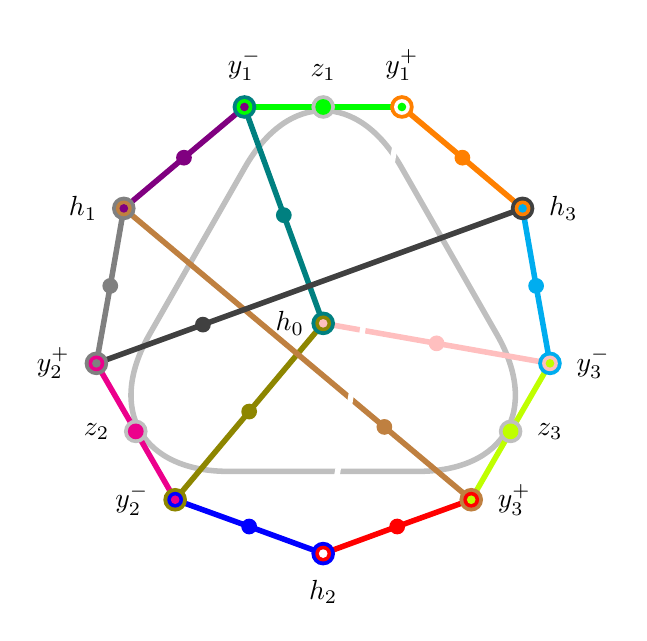
\begin{tikzpicture}  [scale=0.4]

\newdimen\ms
\ms=0.1cm

\tikzstyle{every path}=[line width=2pt]
\tikzstyle{c3}=[circle,inner sep={\ms/8},minimum size=3*\ms]
\tikzstyle{c2}=[circle,inner sep={\ms/8},minimum size=2*\ms]
\tikzstyle{c1}=[circle,inner sep={\ms/8},minimum size=1.1*\ms]



		% Define positions of all observables
		\path
     (-2.50, 6.87    ) coordinate(2)     % $y_1^-
			  (-6.33,   3.65  ) coordinate(4)    % h_1
			  (-7.20, -1.27   ) coordinate(6)       % y_2^+
			  (-4.70, -5.60   ) coordinate(8)       % y_2^-
			  (0, -7.31       ) coordinate(10)       % h_2
			  (4.70, -5.60    ) coordinate(12)        % y_3^+$
     (7.20, -1.27    ) coordinate(14)       % y_3^-
			  (6.33, 3.65     ) coordinate(16)       % h_3
			  (2.50, 6.87     ) coordinate(18)    % y_1^+

			  (0, 6.87        ) coordinate(1)     % z1
			  (-4.42, 5.26    ) coordinate(3)
			  (-6.76, 1.19    ) coordinate(5)
			  (-5.95, -3.43   ) coordinate(7)     % z2
			  (-2.35, -6.45   ) coordinate(9)
     (2.35, -6.45    ) coordinate(11)
			  (5.95,-3.43     ) coordinate(13)    % z3
			  (6.76, 1.19     ) coordinate(15)
		   (4.42, 5.26     ) coordinate(17)

     (0,0) coordinate(19)


(0, 9.3       ) coordinate(20)     % ze1
			  (-8, -4.7    ) coordinate(21)     % ze2
			  (8,-4.7    ) coordinate(22)    % ze3


     (-1.25, 3.435 ) coordinate(23)
     (3.60, -0.635 ) coordinate(24)
     (-2.35, -2.80 ) coordinate(25)
% h1={-6.33,   3.65  }; h3p={4.70, -5.60    } ; h1d2=  (h1+h3p )/2 ; c1=  (h1d2+h3p )/2
     (1.9425, -3.2875) coordinate(26)
% h2={0, -7.31    }; h1p={2.50, 6.87   } ; h2d2=  (h2+h1p )/2 ; c2=  (h2d2+h1p )/2
     (1.875, 3.325) coordinate(27)
% h3={6.33, 3.65    }; h2p={-7.20, -1.27    } ; h3d2=  (h3+h2p )/2 ; c3=  (h3d2+h2p )/2
     (-3.8175, -0.04) coordinate(28)
;

%(4.70-6.33,   3.65  -5.60   ) coordinate(4)    % h_1

	
		% Draw all the context curves
		
\draw [rounded corners=20mm,color=lightgray]     (20) -- (21) -- (22) --  cycle;


\draw [color=green] (18) -- (1) -- (2);
\draw [color=violet] (2) -- (3) -- (4);
\draw [color=gray] (4) -- (5) -- (6);
\draw [color=magenta] (6) -- (7) -- (8);
\draw [color=blue] (8) -- (9) -- (10);
\draw [color=red] (10) -- (11) -- (12) ;

\draw [color=lime] (12) -- (13) -- (14);
\draw [color=cyan] (14) -- (15) -- (16);
\draw [color=orange] (16) -- (17) -- (18);

\draw [color=teal] (19) -- (2);
\draw [color=olive] (19) -- (8);
\draw [color=pink] (19) -- (14);

\draw [color=brown] (4) -- (12);
\draw [color=white] (10) -- (18);
\draw [color=darkgray] (16) -- (6);





%\draw [color=lightgray](0,0) circle (6.87);



\draw (19) coordinate[c3,fill=teal];
\draw (19) coordinate[c2,fill=olive];
\draw (19) coordinate[c1,fill=pink,label=180:$h_0$];


\draw (1)  coordinate[c3,fill=lightgray,label=90:$z_1$];
\draw (1)  coordinate[c2,fill=green];

\draw (2)  coordinate[c3,fill=teal,label=90:$y_1^-$];
\draw (2)  coordinate[c2,fill=green];
\draw (2)  coordinate[c1,fill=violet];

\draw (3)  coordinate[c2,fill=violet];

\draw (4)  coordinate[c3,fill=gray,label=180:$h_1$];
\draw (4)  coordinate[c2,fill=brown];
\draw (4)  coordinate[c1,fill=violet];

\draw (5)  coordinate[c2,fill=gray,label=0:$ $];

\draw (6)  coordinate[c3,fill=darkgray,fill=gray,label=180:$y_2^+$];
\draw (6)  coordinate[c2,fill=magenta];
\draw (6)  coordinate[c1,fill=gray];

\draw (7)  coordinate[c3,fill=lightgray,label=180:$z_2$];
\draw (7)  coordinate[c2,fill=magenta];

\draw (8)  coordinate[c3,fill=olive,label=180:$y_2^-$];
\draw (8)  coordinate[c2,fill=blue];
\draw (8)  coordinate[c1,fill=magenta];

\draw (9)  coordinate[c2,fill=blue,label=0:$ $];

\draw (10) coordinate[c3,fill=blue,label=270:$h_2$];
\draw (10) coordinate[c2,fill=red];
\draw (10) coordinate[c1,fill=white];

\draw (11) coordinate[c2,fill=red,label=0:$ $];

\draw (12) coordinate[c3,fill=brown,label=0:$y_3^+$];
\draw (12) coordinate[c2,fill=red];
\draw (12) coordinate[c1,fill=lime];

\draw (13) coordinate[c3,fill=lightgray,label=0:$z_3$];
\draw (13) coordinate[c2,fill=lime];

\draw (14) coordinate[c3,fill=cyan,label=0:$y_3^-$];
\draw (14) coordinate[c2,fill=pink];
\draw (14) coordinate[c1,fill=lime];

\draw (15) coordinate[c2,fill=cyan,label=0:$ $];

\draw (16) coordinate[c3,fill=darkgray,label=0:$h_3$];
\draw (16) coordinate[c2,fill=orange];
\draw (16) coordinate[c1,fill=cyan];

\draw (17) coordinate[c2,fill=orange,label=0:$ $];

\draw (18) coordinate[c3,fill=orange,label=90:$y_1^+$];
\draw (18) coordinate[c2,fill=white];
\draw (18) coordinate[c1,fill=green];

\draw (23) coordinate[c2,fill=teal];
\draw (24) coordinate[c2,fill=pink];
\draw (25) coordinate[c2,fill=olive];
\draw (26) coordinate[c2,fill=brown];
\draw (27) coordinate[c2,fill=white];
\draw (28) coordinate[c2,fill=darkgray];


		\end{tikzpicture}

 \end{center}
\end{frame}


\begin{frame}[fragile]{Example IV:  True (1) implies true (1) logic (Kochen{\&}Specker, 1967)}

 \begin{center}
%%
%%
%%
%%
%%TexCad Options
%%\grade{\off}
%%\emlines{\off}
%%\beziermacro{\off}
%%\reduce{\on}
%%\snapping{\off}
%%\quality{0.20}
%%\graddiff{0.01}
%%\snapasp{1}
%%\zoom{1.00}
%\unitlength 0.45mm
%%\allinethickness{1pt} %\thicklines %\linethickness{1pt}
%\allinethickness{2pt}
%\begin{picture}(168.00,80.00)
%\put(25.00,7.33){\color{gray}\line(1,0){60.00}}
%\put(25.00,47.33){\color{red}\line(1,0){60.00}}
%\put(55.00,7.33){\color{cyan}\line(0,1){40.00}}
%\put(25.00,7.33){\color{blue}\line(-1,1){20.00}}
%\put(5.00,27.33){\color{green}\line(1,1){20.00}}
%\put(85.00,7.33){\color{magenta}\line(1,1){20.00}}
%\put(105.00,27.33){\color{orange}\line(-1,1){20.00}}
%\put(134.50,27.33){\color{violet}\line(0,-1){20.00}}
%%
%\put(105.00,27.33){\color{pink}\line(1,0){60.00}}
%\put(69, 27.33){\color{violet}\oval(130, 80)[t]}
%%{\color{violet}\qbezier(5,27.33)(32.5,140)(134.76,27.33)}
%%
%\put(134.50,0){\makebox(0,0)[rc]{$b_7$}}
%\put(24.67,55.00){\makebox(0,0)[rc]{$a_3$}}
%\put(55.33,55.00){\makebox(0,0)[cc]{$a_4$}}
%\put(85.33,55.00){\makebox(0,0)[lc]{$a_5$}}
%\put(27.00,37.33){\makebox(0,0)[rc]{$a_2$}}
%\put(99.33,40.00){\makebox(0,0)[lc]{$a_6$}}
%\put(0.00,27.33){\makebox(0,0)[rc]{$a_1$}}
%\put(113.00,32.33){\makebox(0,0)[lc]{$a_7$}}
%\put(60.33,31.33){\makebox(0,0)[lc]{$a_{13}$}}
%\put(9.00,13.33){\makebox(0,0)[rc]{$a_{12}$}}
%\put(99.67,13.33){\makebox(0,0)[lc]{$a_8$}}
%\put(24.67,0){\makebox(0,0)[rc]{$a_{11}$}}
%\put(55.33,0){\makebox(0,0)[cc]{$a_{10}$}}
%\put(85.33,0){\makebox(0,0)[lc]{$a_9$}}
%\put(134.50,7){\color{violet}\circle{1.00}}
%\put(134.50,7){\color{violet}\circle{2.00}}
%\put(15.00,17.09){\color{blue}\circle{1.00}}
%\put(15.00,17.09){\color{blue}\circle{2.00}}
%\put(25.00,7.33){\color{blue}\circle{1.00}}
%\put(25.00,7.33){\color{blue}\circle{2.00}}
%\put(25.00,7.33){\color{gray}\circle{3.00}}
%\put(55.00,27.33){\color{cyan}\circle{1.00}}
%\put(55.00,27.33){\color{cyan}\circle{2.00}}
%\put(85.00,7.33){\color{gray}\circle{1.00}}
%\put(85.00,7.33){\color{gray}\circle{2.00}}
%\put(85.00,7.33){\color{magenta}\circle{3.00}}
%\put(95.00,17.33){\color{magenta}\circle{1.00}}
%\put(95.00,17.33){\color{magenta}\circle{2.00}}
%\put(5.00,27.33){\color{green}\circle{1.00}}
%\put(5.00,27.33){\color{green}\circle{2.00}}
%\put(5.00,27.33){\color{green}\circle{3.00}}
%\put(5.00,27.33){\color{blue}\circle{3.0}}
%\put(5.00,27.33){\color{violet}\circle{5.00}}
%\put(15.00,37.33){\color{green}\circle{1.00}}
%\put(15.00,37.33){\color{green}\circle{2.00}}
%\put(25.00,47.33){\color{green}\circle{1.00}}
%\put(25.00,47.33){\color{green}\circle{2.00}}
%\put(25.00,47.33){\color{red}\circle{3.00}}
%\put(55.00,47.33){\color{red}\circle{1.00}}
%\put(55.00,47.33){\color{red}\circle{2.00}}
%\put(55.00,47.33){\color{cyan}\circle{3.00}}
%\put(85.00,47.33){\color{red}\circle{1.00}}
%\put(85.00,47.33){\color{red}\circle{2.00}}
%\put(85.00,47.33){\color{orange}\circle{3.00}}
%\put(55.00,7.33){\color{gray}\circle{1.00}}
%\put(55.00,7.33){\color{gray}\circle{2.00}}
%\put(55.00,7.33){\color{cyan}\circle{3.00}}
%\put(105,27.33){\color{orange}\circle{1.00}}
%\put(105,27.33){\color{orange}\circle{2.00}}
%\put(105,27.33){\color{magenta}\circle{3.00}}
%\put(105,27.33){\color{pink}\circle{5.00}}
%\put(95.00,37.33){\color{orange}\circle{1.00}}
%\put(95.00,37.33){\color{orange}\circle{2.00}}
%
%\put(165,27.33){\color{pink}\circle{1.00}}
%\put(165,27.33){\color{pink}\circle{2.00}}
%\put(135,27.33){\color{pink}\circle{1.00}}
%\put(134.76,27.33){\color{pink}\circle{2.00}}
%\put(134.76,27.33){\color{violet}\circle{3.00}}
%\put(140.00,32.33){\makebox(0,0)[lc]{$c$}}
%\put(168.00,27.33){\makebox(0,0)[lc]{$b_1$}}
%\end{picture}
%
%
% This is a LaTeX picture output by TeXCAD.
% File name: [1.pic].
% Version of TeXCAD: 4.3
% Reference / build: 30-Jun-2012 (rev. 105)
% For new versions, check: http://texcad.sf.net/
% Options on the following lines.
%\grade{\off}
%\emlines{\off}
%\epic{\off}
%\beziermacro{\on}
%\reduce{\on}
%\snapping{\off}
%\quality{0.200}
%\graddiff{0.010}
%\snapasp{1}
%\zoom{8.0000}
%\unitlength 1mm % = 2.845pt
%\linethickness{0.4pt}
\unitlength 0.55mm
\allinethickness{2pt}
\ifx\plotpoint\undefined\newsavebox{\plotpoint}\fi % GNUPLOT compatibility
\begin{picture}(152,120)(0,0)
%
\put(15.455,85.051){\color{gray}\line(0,-1){60}}
%\put(144.545,85.051){\color{gray}\line(0,-1){60}}
\put(55.455,85.051){\color{red}\line(0,-1){60}}
%\put(104.545,85.051){\color{red}\line(0,-1){60}}
\put(15.455,55.051){\color{cyan}\line(1,0){40}}
%\put(144.545,55.051){\color{cyan}\line(-1,0){40}}
\put(15.455,85.051){\color{blue}\line(1,1){20}}
%\put(144.545,85.051){\color{blue}\line(-1,1){20}}
\put(35.455,105.051){\color{green}\line(1,-1){20}}
%\put(124.545,105.051){\color{green}\line(-1,-1){20}}
\put(15.455,25.051){\color{magenta}\line(1,-1){20}}
%\put(144.545,25.051){\color{magenta}\line(-1,-1){20}}
\put(35.455,5.051){\color{orange}\line(1,1){20}}
%\put(124.545,5.051){\color{orange}\line(-1,1){20}}
%
%
\color{pink}\qbezier(35.5,5.25)(68,5.625)(80,55)
\color{violet}\qbezier(124.5,5.25)(92,5.625)(80,55)
\color{violet}\qbezier(35.5,104.5)(68,104.125)(80,54.75)
\color{pink}\qbezier(124.5,104.5)(92,104.125)(80,54.75)
{\color{yellow}
%
\put(62.125,80.381){\makebox(0,0)[b]{$a_3$}}
%\put(98.875,80.381){\makebox(0,0)[b]{$b_3$}}
\put(62.125,54.721){\makebox(0,0)[]{$a_4$}}
%\put(98.875,54.721){\makebox(0,0)[]{$b_4$}}
\put(62.125,26.721){\makebox(0,0)[t]{$a_5$}}
%\put(98.875,26.721){\makebox(0,0)[t]{$b_5$}}
\put(43.125,85.051){\makebox(0,0)[b]{$a_2$}}
%\put(116.875,85.051){\makebox(0,0)[b]{$b_2$}}
\put(43.125,22.721){\makebox(0,0)[t]{$a_6$}}
%\put(116.875,22.721){\makebox(0,0)[t]{$b_6$}}
\put(34.455,110.051){\makebox(0,0)[b]{$a_1$}}
 \put(125.545,110.051){\makebox(0,0)[b]{$b_1$}}
\put(34.455,0){\makebox(0,0)[t]{$a_7$}}
 \put(125.545,0){\makebox(0,0)[t]{$b_7$}}
\put(35,49.721){\makebox(0,0)[t]{$a_{13}$}}
%\put(125,49.721){\makebox(0,0)[t]{$b_{13}$}}
\put(21.455,101.051){\makebox(0,0)[b]{$a_{12}$}}
%\put(138.545,101.051){\makebox(0,0)[b]{$b_{12}$}}
\put(21.455,10.381){\makebox(0,0)[t]{$a_8$}}
%\put(138.545,10.381){\makebox(0,0)[t]{$b_8$}}
\put(8.075,85.381){\makebox(0,0)[b]{$a_{11}$}}
%\put(151.925,85.381){\makebox(0,0)[b]{$b_{11}$}}
\put(8.075,54.721){\makebox(0,0)[]{$a_{10}$}}
%\put(151.925,54.721){\makebox(0,0)[]{$b_{10}$}}
\put(8.075,24.721){\makebox(0,0)[t]{$a_9$}}
%\put(151.925,24.721){\makebox(0,0)[t]{$b_9$}}
\put(85,55){\makebox(0,0)[t]{$c$}}
\put(25.215,95.051){\color{blue}\circle{1}}
%\put(134.785,95.051){\color{blue}\circle{1}}
\put(25.215,95.051){\color{blue}\circle{2}}
%\put(134.785,95.051){\color{blue}\circle{2}}
\put(15.455,85.051){\color{blue}\circle{1}}
%\put(144.545,85.051){\color{blue}\circle{1}}
\put(15.455,85.051){\color{blue}\circle{2}}
%\put(144.545,85.051){\color{blue}\circle{2}}
\put(15.455,85.051){\color{gray}\circle{3}}
%\put(144.545,85.051){\color{gray}\circle{3}}
\put(35.455,55.051){\color{cyan}\circle{1}}
%%\put(124.545,55.051){\color{cyan}\circle{1}}
 \put(35.455,55.051){\color{cyan}\circle{2}}
%%\put(124.545,55.051){\color{cyan}\circle{2}}
\put(15.455,25.051){\color{gray}\circle{1}}
%\put(144.545,25.051){\color{gray}\circle{1}}
\put(15.455,25.051){\color{gray}\circle{2}}
%\put(144.545,25.051){\color{gray}\circle{2}}
\put(15.455,25.051){\color{magenta}\circle{3}}
%\put(144.545,25.051){\color{magenta}\circle{3}}
\put(25.455,15.051){\color{magenta}\circle{1}}
%\put(134.545,15.051){\color{magenta}\circle{1}}
\put(25.455,15.051){\color{magenta}\circle{2}}
%\put(134.545,15.051){\color{magenta}\circle{2}}
\put(35.455,105.051){\color{blue}\circle{1}}
%\put(124.545,105.051){\color{blue}\circle{1}}
\put(35.455,105.051){\color{blue}\circle{1}}
%\put(124.545,105.051){\color{blue}\circle{1}}
\put(35.455,105.051){\color{green}\circle{3}}
%\put(124.545,105.051){\color{green}\circle{3}}
\put(35.455,105.051){\color{violet}\circle{5}}
\put(124.545,105){\color{pink}\circle{3}}  %$$$
\put(124.545,105){\color{pink}\circle{1}}  %$$$
\put(45.455,95.051){\color{green}\circle{1}}
%\put(114.545,95.051){\color{green}\circle{1}}
\put(45.455,95.051){\color{green}\circle{2}}
%\put(114.545,95.051){\color{green}\circle{2}}
\put(55.455,85.051){\color{green}\circle{1}}
%\put(104.545,85.051){\color{green}\circle{1}}
\put(55.455,85.051){\color{green}\circle{2}}
%\put(104.545,85.051){\color{green}\circle{2}}
\put(55.455,85.051){\color{red}\circle{3}}
% \put(104.545,85.051){\color{red}\circle{3}}
 \put(55.455,55.051){\color{cyan}\circle{1}}
 %\put(104.545,55.051){\color{cyan}\circle{1}}
 \put(55.455,55.051){\color{cyan}\circle{3}}
 %\put(104.545,55.051){\color{cyan}\circle{1}}
\put(55.455,55.051){\color{red}\circle{3}}
%\put(104.545,55.051){\color{red}\circle{3}}
\put(55.455,25.051){\color{red}\circle{1}}
%\put(104.545,25.051){\color{red}\circle{1}}
\put(55.455,25.051){\color{red}\circle{2}}
%\put(104.545,25.051){\color{red}\circle{2}}
\put(55.455,25.051){\color{orange}\circle{3}}
%\put(104.545,25.051){\color{orange}\circle{3}}
\put(15.455,55.051){\color{cyan}\circle{1}}
%\put(144.545,55.051){\color{cyan}\circle{1}}
\put(15.455,55.051){\color{cyan}\circle{2}}
%\put(144.545,55.051){\color{cyan}\circle{2}}
\put(15.455,55.051){\color{gray}\circle{3}}
%\put(144.545,55.051){\color{gray}\circle{3}}
\put(35.455,5.291){\color{orange}\circle{1}}
%\put(124.545,5.291){\color{orange}\circle{1}}
\put(35.455,5.291){\color{orange}\circle{2}}
%\put(124.545,5.291){\color{orange}\circle{2}}
\put(35.455,5.291){\color{magenta}\circle{3}}
%\put(124.545,5.291){\color{magenta}\circle{3}}
\put(35.455,5.291){\color{pink}\circle{5}}
\put(124.545,5.291){\color{violet}\circle{3}}  %$$$
\put(124.545,5.291){\color{violet}\circle{1}}  %$$$
\put(45.455,15.051){\color{orange}\circle{1}}
%\put(114.545,15.051){\color{orange}\circle{1}}
\put(45.455,15.051){\color{orange}\circle{2}}
%\put(114.545,15.051){\color{orange}\circle{2}}
\put(80,55){\color{pink}\circle{1}}
\put(80,55){\color{violet}\circle{3}}
}
\end{picture}
 \end{center}
\end{frame}



\begin{frame}[fragile]{Example V: Combo of two linked Specker bug logics inducing
a non-separating set of two-valued states}

 \begin{center}
% This is a LaTeX picture output by TeXCAD.
% File name: [1.pic].
% Version of TeXCAD: 4.3
% Reference / build: 30-Jun-2012 (rev. 105)
% For new versions, check: http://texcad.sf.net/
% Options on the following lines.
%\grade{\off}
%\emlines{\off}
%\epic{\off}
%\beziermacro{\on}
%\reduce{\on}
%\snapping{\off}
%\quality{0.200}
%\graddiff{0.010}
%\snapasp{1}
%\zoom{8.0000}
%\unitlength 1mm % = 2.845pt
%\linethickness{0.4pt}
\unitlength 0.55mm
\allinethickness{2pt}
\ifx\plotpoint\undefined\newsavebox{\plotpoint}\fi % GNUPLOT compatibility
\begin{picture}(152,120)(0,0)
%
\put(15.455,85.051){\color{gray}\line(0,-1){60}}
\put(144.545,85.051){\color{gray}\line(0,-1){60}}
\put(55.455,85.051){\color{red}\line(0,-1){60}}
\put(104.545,85.051){\color{red}\line(0,-1){60}}
\put(15.455,55.051){\color{cyan}\line(1,0){40}}
\put(144.545,55.051){\color{cyan}\line(-1,0){40}}
\put(15.455,85.051){\color{blue}\line(1,1){20}}
\put(144.545,85.051){\color{blue}\line(-1,1){20}}
\put(35.455,105.051){\color{green}\line(1,-1){20}}
\put(124.545,105.051){\color{green}\line(-1,-1){20}}
\put(15.455,25.051){\color{magenta}\line(1,-1){20}}
\put(144.545,25.051){\color{magenta}\line(-1,-1){20}}
\put(35.455,5.051){\color{orange}\line(1,1){20}}
\put(124.545,5.051){\color{orange}\line(-1,1){20}}
%
%
\color{pink}\qbezier(35.5,5.25)(68,5.625)(80,55)
\color{violet}\qbezier(124.5,5.25)(92,5.625)(80,55)
\color{violet}\qbezier(35.5,104.5)(68,104.125)(80,54.75)
\color{pink}\qbezier(124.5,104.5)(92,104.125)(80,54.75)
{\color{yellow}
%
\put(62.125,80.381){\makebox(0,0)[b]{$a_3$}}
\put(98.875,80.381){\makebox(0,0)[b]{$b_3$}}
\put(62.125,54.721){\makebox(0,0)[]{$a_4$}}
\put(98.875,54.721){\makebox(0,0)[]{$b_4$}}
\put(62.125,26.721){\makebox(0,0)[t]{$a_5$}}
\put(98.875,26.721){\makebox(0,0)[t]{$b_5$}}
\put(43.125,85.051){\makebox(0,0)[b]{$a_2$}}
\put(116.875,85.051){\makebox(0,0)[b]{$b_2$}}
\put(43.125,22.721){\makebox(0,0)[t]{$a_6$}}
\put(116.875,22.721){\makebox(0,0)[t]{$b_6$}}
\put(34.455,110.051){\makebox(0,0)[b]{$a_1$}}
\put(125.545,110.051){\makebox(0,0)[b]{$b_1$}}
\put(34.455,0){\makebox(0,0)[t]{$a_7$}}
\put(125.545,0){\makebox(0,0)[t]{$b_7$}}
\put(35,49.721){\makebox(0,0)[t]{$a_{13}$}}
\put(125,49.721){\makebox(0,0)[t]{$b_{13}$}}
\put(21.455,101.051){\makebox(0,0)[b]{$a_{12}$}}
\put(138.545,101.051){\makebox(0,0)[b]{$b_{12}$}}
\put(21.455,10.381){\makebox(0,0)[t]{$a_8$}}
\put(138.545,10.381){\makebox(0,0)[t]{$b_8$}}
\put(8.075,85.381){\makebox(0,0)[b]{$a_{11}$}}
\put(151.925,85.381){\makebox(0,0)[b]{$b_{11}$}}
\put(8.075,54.721){\makebox(0,0)[]{$a_{10}$}}
\put(151.925,54.721){\makebox(0,0)[]{$b_{10}$}}
\put(8.075,24.721){\makebox(0,0)[t]{$a_9$}}
\put(151.925,24.721){\makebox(0,0)[t]{$b_9$}}
\put(85,55){\makebox(0,0)[t]{$c$}}
\put(25.215,95.051){\color{blue}\circle{1}}
\put(134.785,95.051){\color{blue}\circle{1}}
\put(25.215,95.051){\color{blue}\circle{2}}
\put(134.785,95.051){\color{blue}\circle{2}}
\put(15.455,85.051){\color{blue}\circle{1}}
\put(144.545,85.051){\color{blue}\circle{1}}
\put(15.455,85.051){\color{blue}\circle{2}}
\put(144.545,85.051){\color{blue}\circle{2}}
\put(15.455,85.051){\color{gray}\circle{3}}
\put(144.545,85.051){\color{gray}\circle{3}}
 \put(35.455,55.051){\color{cyan}\circle{1}}
 \put(124.545,55.051){\color{cyan}\circle{1}}
 \put(35.455,55.051){\color{cyan}\circle{2}}
 \put(124.545,55.051){\color{cyan}\circle{2}}
\put(15.455,25.051){\color{gray}\circle{1}}
\put(144.545,25.051){\color{gray}\circle{1}}
\put(15.455,25.051){\color{gray}\circle{2}}
\put(144.545,25.051){\color{gray}\circle{2}}
\put(15.455,25.051){\color{magenta}\circle{3}}
\put(144.545,25.051){\color{magenta}\circle{3}}
\put(25.455,15.051){\color{magenta}\circle{1}}
\put(134.545,15.051){\color{magenta}\circle{1}}
\put(25.455,15.051){\color{magenta}\circle{2}}
\put(134.545,15.051){\color{magenta}\circle{2}}
\put(35.455,105.051){\color{blue}\circle{1}}
\put(124.545,105.051){\color{blue}\circle{1}}
\put(35.455,105.051){\color{blue}\circle{1}}
\put(124.545,105.051){\color{blue}\circle{1}}
\put(35.455,105.051){\color{green}\circle{3}}
\put(124.545,105.051){\color{green}\circle{3}}
\put(35.455,105.051){\color{violet}\circle{5}}
\put(124.545,105.051){\color{pink}\circle{5}}
\put(45.455,95.051){\color{green}\circle{1}}
\put(114.545,95.051){\color{green}\circle{1}}
\put(45.455,95.051){\color{green}\circle{2}}
\put(114.545,95.051){\color{green}\circle{2}}
\put(55.455,85.051){\color{green}\circle{1}}
\put(104.545,85.051){\color{green}\circle{1}}
\put(55.455,85.051){\color{green}\circle{2}}
\put(104.545,85.051){\color{green}\circle{2}}
\put(55.455,85.051){\color{red}\circle{3}}
\put(104.545,85.051){\color{red}\circle{3}}
 \put(55.455,55.051){\color{cyan}\circle{1}}
 \put(55.455,55.051){\color{cyan}\circle{3}}
 \put(104.545,55.051){\color{cyan}\circle{1}}
 \put(104.545,55.051){\color{cyan}\circle{3}}
\put(55.455,55.051){\color{red}\circle{3}}
\put(104.545,55.051){\color{red}\circle{3}}
\put(55.455,25.051){\color{red}\circle{1}}
\put(104.545,25.051){\color{red}\circle{1}}
\put(55.455,25.051){\color{red}\circle{2}}
\put(104.545,25.051){\color{red}\circle{2}}
\put(55.455,25.051){\color{orange}\circle{3}}
\put(104.545,25.051){\color{orange}\circle{3}}
\put(15.455,55.051){\color{cyan}\circle{1}}
\put(144.545,55.051){\color{cyan}\circle{1}}
\put(15.455,55.051){\color{cyan}\circle{2}}
\put(144.545,55.051){\color{cyan}\circle{2}}
\put(15.455,55.051){\color{gray}\circle{3}}
\put(144.545,55.051){\color{gray}\circle{3}}
\put(35.455,5.291){\color{orange}\circle{1}}
\put(124.545,5.291){\color{orange}\circle{1}}
\put(35.455,5.291){\color{orange}\circle{2}}
\put(124.545,5.291){\color{orange}\circle{2}}
\put(35.455,5.291){\color{magenta}\circle{3}}
\put(124.545,5.291){\color{magenta}\circle{3}}
\put(35.455,5.291){\color{pink}\circle{5}}
\put(124.545,5.291){\color{violet}\circle{5}}
\put(45.455,15.051){\color{orange}\circle{1}}
\put(114.545,15.051){\color{orange}\circle{1}}
\put(45.455,15.051){\color{orange}\circle{2}}
\put(114.545,15.051){\color{orange}\circle{2}}
\put(80,55){\color{pink}\circle{1}}
\put(80,55){\color{violet}\circle{3}}
}
\end{picture}
 \end{center}
\end{frame}


\begin{frame}[fragile]{Quantum challenge \& outlook: Hilbert logics without a two-valued states (Gleason 1957, Specker 1960)}

\begin{itemize}
%\pause
\item
In such situations the classical strategy to build probabilities from two-valued states fails entirely.

\item
Gleason suggested a new strategy, which, for pure states (formalizable as normalized vector) can be based upon the
``Pythagorean (theorem) view from orthonormal bases.''

\item
In such situations, value indefiniteness rulez (Pitowsky 1998,2004; Abbott,Calude,Conder,KS 2012,2014, arXiv:1503.01985,
   doi 10.1063/1.49316582014 2015)

\item
more ``exotic'' phenomena -- e.g. demanding Wright's ``exotic'' dispersionless state?

\end{itemize}



\end{frame}

\frame{

\centerline{\huge {\color{yellow} Thank you for your attention!}}

\begin{center}\color{orange}
$\widetilde{\qquad \qquad }$
$\widetilde{\qquad \qquad}$
$\widetilde{\qquad \qquad }$
\end{center}
 }
 \end{document}





\begin{frame}[fragile]{Example I}

\begin{center}

\end{center}

\end{frame}

 \frame{
 \frametitle{}

 }

